\synctex=1
\documentclass[dvipdfmx,10pt, a4j]{jarticle}
%----------------------------------------------------------
%パッケージ読み込み
\usepackage{amsmath}
\usepackage{amssymb}
\usepackage{amsthm} %定理環境の拡張
\usepackage{ascmac}
\usepackage{bm}
\usepackage{cases}
\usepackage{comment} %非表示にするためのコメント
\usepackage{enumerate}
\usepackage{float} %画像をその場に表示.[h]の代わりに[H]
\usepackage{graphicx} % eps 形式の図版取り込みのため
\usepackage{mathrsfs}
\usepackage{url}
\usepackage[dvipdfmx]{hyperref}
\usepackage{color}
%----------------------------------------------------------

%----------------------------------------------------------
%命題関係の定義
\theoremstyle{definition}
\newtheorem{definition}{定義}[section]
\newtheorem{theorem}{定理}[section]
\newtheorem{proposition}[theorem]{命題}
\newtheorem{lemma}[theorem]{補題}
\newtheorem{col}[theorem]{系}
\newtheorem{example}{例}[section]
\newtheorem{remark}{注意}[section]
%----------------------------------------------------------

%タイトル・著者===================================================
\title{第8回 数理統計 レポート}
\author{小森 一輝}
%=================================================================

%本文開始=========================================================
\begin{document}

\maketitle

%カウンタ--------------------------------------------------
\setcounter{section}{2}
%\setcounter{subsection}{0}
%\setcounter{subsubsection}{0}
%\setcounter{theorem}{0}

%----------------------------------------------------------定義3.9
\noindent
\textbf{定義 3.9.} 期待値\\
\begin{enumerate}[i)]
    \item $確率変数X が離散型の場合, Xの確率関数f_Xが \fbox{$\sum_{i=1}^{\infty}{|x_i| f_X(x_i)} < \infty$}$
          $(D = \{x_i| i = 1,2,\dots \})を満たすとき, Xの \textbf{期待値(expected value) $\mu$ }を次式で定義する.$\\
          \begin{align*}
              \mu = E(X) = \sum_{i=1}^{\infty}{x_i f_X(x_i)} \\
          \end{align*}
    \item $確率変数Xが連続型の場合, Xの確率変数 f_X が \fbox{$\int_{-\infty}^{\infty}{|x|f_X(x)dx} < \infty$} を$
          $満たすとき,Xの \textbf{期待値 $\mu$}を次式で定義する.$\\
          \begin{align*}
              \mu = E(X) = \int_{-\infty}^{\infty}{xf_X(x)dx} \\
          \end{align*}
          $確率変数Xの期待値は \textbf{平均値(mean)}と呼ばれることもある.$\\
\end{enumerate}
%---------------以下補足
\begin{itembox}[l]{注}
    常に期待値は存在するとは限らない. \\
    $E_{分布を表す}(確率変数)$\\
    $E_{\textcolor{red}{X}}(\textcolor{blue}{X}) = \int \textcolor{blue}{x}f_{\textcolor{red}{X}}(\textcolor{green}{t})d\textcolor{green}{t}$\\
\end{itembox}\\

%----------------------------------------------------------定理3.18
\noindent
\textbf{定理 3.18.} $X, Yを確率変数とし, Y=h(X)とする. ただし, h: \mathbb{R} \to \mathbb{R} は微分可能な単調関数とする.$
$このとき, E(Y) < \infty であれば, 以下が成り立つ.$\\
\begin{align*}
    E(Y) = E(h(X)) \\
\end{align*}

%----------------------------------------------------------命題3.19
\noindent
\textbf{命題 3.19.} 期待値の性質\\
$\phi, \psi: \mathbb{R} \to \mathbb{R} をボレル関数とし, a, b \in \mathbb{R} を定数とする.$
$このとき, E(\phi(X)) < \infty, E(\psi(X)) < \infty であれば, 以下が成り立つ.$\\
\begin{align*}
     & E(a\phi(X) + b\psi(X)) = aE(\phi(X)) + bE(\psi(X)) \\
     & |E(\phi(X)| \leq E(|\phi(X)|)                      \\
\end{align*}
\begin{proof}離散型\\
    \begin{align*}
        E_X(a \phi(X) + b\psi(X)) & = \sum_{i=1}^{\infty}{(a \phi(X) + b\psi(X))}f_X(x_i) \\
                                  & = a \sum \phi(X)f_X(x_i) + b \sum \psi(X)f_X(x_i)     \\
                                  & = aE(\phi(X)) + bE(\psi(X))                           \\
    \end{align*}
\end{proof}
\begin{proof}連続型\\
    \begin{align*}
        E_X(a \phi(X) + b\psi(X)) & = \int{(a \phi(X) + b\psi(X))}f_X(x_i)                \\
                                  & = a \int \phi(X)f_X(x_i)dx + b \int \psi(X)f_X(x_i)dx \\
                                  & = aE(\phi(X)) + bE(\psi(X))                           \\
    \end{align*}
\end{proof}
\begin{proof}
    \begin{align*}
         & |\sum f(x_i)| \leq \sum|f(x_i)| \\
         & |\int f(x_i)| \leq \int|f(x_i)| \\
    \end{align*}
    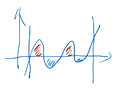
\includegraphics[width=7.0cm]{D_8/img_1.png}
    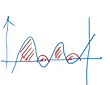
\includegraphics[width=7.0cm]{D_8/img_2.png}
\end{proof}

%----------------------------------------------------------定義3.10
\noindent
\textbf{定義 3.10.} 分散, 標準偏差\\
\begin{enumerate}[i)]
    \item $確率変数X が離散型の場合, X の確率関数 f_X が \sum_{i=1}^{\infty}{x_i^{2}f_X(x_i)} < \infty (D= \{x_i \mid i=1,2,\dots \})$
          $を満たすとき, Xの \textbf{分散(varaiance)}を次式で定義し, \sigma^{2}と記す.$\\
          \begin{align*}
              \sigma^{2} = V(X) = E((X-\mu)^2) = \sum_{i=1}^{\infty}{(x_i - \mu)^{2}f_X(x_i)} \\
          \end{align*}
    \item $確率変数Xが連続型の場合, X の確率密度関数f_X が \int_{-\infty}^{\infty}{x^2f_X(x)dx} < \infty を満たすとき,$
          $Xの \textbf{分散}を次式で定義し, 同じく \sigma^{2}と記す.$\\
          \begin{align*}
              \sigma^{2} = V(X) = E((X-\mu)^2) = \int_{-\infty}^{\infty}{(x-\mu)^2f_X(x)dx} \\
          \end{align*}
    \item $確率変数X の \textbf{標準偏差(standard deviation)} を次式で定義し, \sigma と記す.$\\
          \begin{align*}
              \sigma = \sqrt{V(X)} \\
          \end{align*}
          $すなわち, 標準偏差は分散の正の平方根である.$\\
\end{enumerate}

\newpage
%----------------------------------------------------------例3.4
\noindent
\textbf{例 3.4.} $確率変数X の期待値, 分散について, 次式が成り立つ.$\\
\begin{align*}
     & E(aX + b) = aE(X) + b, \qquad V(aX + b) = a^2V(X) \\
     & V(X) = E(X^2) - (E(X))^2                          \\
\end{align*}
\begin{proof}
    \begin{align*}連続型                                       \\
        E(aX + b) & = \int (ax+b)f(x)dx              \\
                  & =a \int xf(x)dx + b \int xf(x)dx \\
                  & = aE(X)+b                        \\
    \end{align*}
    ※離散型も同様\\
\end{proof}
\begin{proof}
    \begin{align*}
        V(aX + b) & = E((aX + b - E(aX+b))^2)                     \\
                  & =E((aX+b-aE(X)+b)^2)                          \\
                  & = E(a^2(X-E(X))^2) = a^2E((X-E(X))^2)=a^2V(X) \\
    \end{align*}
\end{proof}
\begin{proof}
    \begin{align*}
        V(X) & = E((X-E(X))^2)                 \\
             & = E(X^2 - 2XE(X) + (E(X))^2)    \\
             & = E(X^2 - 2E(X)E(X) + (E(X))^2) \\
             & = E(X^2) - (E(X))^2             \\
    \end{align*}
\end{proof}
%----------------------------------------------------------例3.5
\noindent
\textbf{例 3.5.} $確率変数X の期待値, 分散について, 次式が成り立つ.$\\
\begin{align*}
     & E(X - \mu) = 0                                                    \\
     & E((X - c)^2) \geq E((X - \mu)^2) = V(X) \qquad (c \in \mathbb{R}) \\
\end{align*}
\begin{proof}
    \begin{align*}
        E(X-\mu) & = E(X) - \mu    \\
                 & = \mu - \mu = 0 \\
    \end{align*}
\end{proof}
\begin{proof}
    \begin{align*}
        左辺 - 右辺 & = E((X -c)^2) - E((X-\mu)^2)                        \\
                    & =E((X-c)^2 - (X-\mu)^2)                             \\
                    & =E(-2cX + c^2 + 2 \mu X - \mu^2)                    \\
                    & =(-2c + 2\mu)E(X) + c^2 -\mu^2                      \\
                    & = -2c\mu + 2 \mu^2 - \mu^2 + c^2 = (c-\mu)^2 \geq 0 \\
                    & 等号成立は c = \mu                                  \\
    \end{align*}
\end{proof}
%---------------以下補足
\begin{itembox}[l]{補足}
    データで以下のようにあらわすことができる.
    \begin{align*}
         & \sum (x_i - \overline{x}) = 0                    \\
         & \sum (x_i -c)^2 \geq \sum (x_i - \overline{x})^2 \\
    \end{align*}
\end{itembox}\\

%----------------------------------------------------------定義3.11
\noindent
\textbf{定義 3.11.} 積率\\
$確率変数Xについて, ある n \in \mathbb{N} に対し, E(X^n) < \infty であれば,$\\
$E(X^n) を\textbf{原点まわりのn次積率(nth \textcolor{red}{moment} about the origin)}, または, \textbf{\fbox{原点積率}(nth origin moment)}という.$\\
$さらに, ある \mu = E(X) が与えられるとき, E((X-\mu)^n)を \textbf{平均周りのn次積率(nth moment about the mean)},$\\
$または, \textbf{\fbox{中心積率}(nth central moment)}という. 以下, \mu_n = E(X^{n}), \; \mu_n^{\prime} = E((X-\mu)^n)と記す.$\\
%---------------以下補足
\begin{itembox}[l]{補足}
    \begin{align*}
         & 原点まわりのn次積率\; :\; \mu_n^{\prime} = E(X^n) \\
         & 平均まわりのn次積率\; : \; \mu_n = E((X-\mu)^n)   \\
         & \mu_1^{\prime} = E(X) = \mu                       \\
         & \mu_2 = V(X) = \sigma^2                           \\
    \end{align*}
\end{itembox}\\

%----------------------------------------------------------定理3.20
\noindent
\textbf{定理 3.20.} 積率の存在\\
$確率変数Xおよび, n(\in \mathbb{N}) に対して, E(X^n) < \infty が成り立てば,$
$0 < k \leq nに対して, E(X^k)が成り立つ. つまり, n次の積率が存在すれば, n次以下の積率も存在する.$\\
\begin{align*}
    \int |x^n|f(x)dx < \infty \rightarrow \int |x^k|f(x)dx < \infty \\
\end{align*}

%----------------------------------------------------------命題3.21
\noindent
\textbf{命題 3.21.} 確率変数Xの積率に関して, 次式が成り立つ. \\
(\textcolor{red}{平均積率を中心積率で表す!!})\\
\begin{align*}
     & \mu_2 = \mu_2^{\prime} - (\mu_1^{\prime})^2                                                                         \\
     & \mu_3 = \mu_3^{\prime} - 3 \mu_1^{\prime} \mu_2^{\prime} + 2(\mu_1^{\prime})^3                                      \\
     & \mu_4 = \mu_4^{\prime} - 4 \mu_1^{\prime} \mu_3^{\prime} + 6(\mu_1^{\prime})^2 \mu_2^{\prime} - 3(\mu_1^{\prime})^4 \\
\end{align*}
\begin{proof}
    \begin{align*}
        V(X) & = E(X^2) - (E(X))^2                   \\
             & = \mu_2^{\prime} - (\mu_1^{\prime})^2 \\
    \end{align*}
\end{proof}
\begin{proof}
    \begin{align*}
        \mu_3 & = E((X- \mu )^3)                                                                                       \\
              & = E(X^3 - 3X^2\mu + 3X\mu^2 - \mu^3)                                                                   \\
              & = E(X^3) -3\mu E(X^2) + 3\mu^2 E(X) - \mu^3                                                            \\
              & = \mu_3^{\prime} - 3\mu_1^{\prime}\mu_2^{\prime} + 3\mu_1^{\prime 2} \mu_1^{\prime} - \mu_1^{\prime 3} \\
              & = \mu_3^{\prime} - 3\mu_1^{\prime}\mu_2^{\prime} + 2 \mu_1^{\prime 2}                                  \\
    \end{align*}
\end{proof}

%----------------------------------------------------------定理3.22
\noindent
\textbf{定理 3.22.} 平均まわりの積率と原点まわりの積率の関係\\
$平均まわりの積率 \mu_k と, 原点まわりの積率 \mu_k^{\prime}には以下の関係が成り立つ.$\\
\begin{align*}
     & \mu_k = \sum_{i=1}^{k}{(-1)^{k-i}}
    \left( \begin{array}{c}
            i \\
            k
        \end{array}
    \right)
    \mu_i^{\prime}(\mu_1^{\prime})^{k-i}  \\
     & \mu_k^{\prime} = \sum_{i=1}^{k}
    \left( \begin{array}{c}
            i \\
            k
        \end{array}
    \right)
    \mu_i(\mu_1^{\prime})^{k-i}           \\
\end{align*}
$ここで, ()は二項係数を表し, 形式的に 0! = 1, \mu_0^{\prime} = 1を仮定している.$\\
\begin{proof}

    \begin{align*}
        \mu_k = E((X-\mu)^k) & = E(\sum_{i=1}^{k}{(-1)^{k-i}
        \left(
        \begin{array}{c}
                i \\
                k
            \end{array}
        \right)
        X^i \mu^{k-i}})                                      \\
                             & = \sum_{i=1}^{k}{(-1)^{k-i}
        \left(
        \begin{array}{c}
                i \\
                k
            \end{array}
        \right)
        E(X^i)(\mu_1^{\prime})^{k-i}}                        \\
                             & = \sum_{i=1}^{k}{(-1)^{k-i}
        \left(
        \begin{array}{c}
                i \\
                k
            \end{array}
        \right)
        \mu_i^{\prime}(\mu_1^{\prime})^{k-i}}                \\
    \end{align*}
\end{proof}
\begin{proof}
    \begin{align*}
        \mu_k^{\prime} & = E(X^k)              \\
                       & =E((X - \mu + \mu)^k) \\
                       & =\sum_{i=1}^{k}
        \left(
        \begin{array}{c}
                i \\
                k
            \end{array}
        \right)
        E((X-\mu)^i)\mu^{k-i}                  \\
                       & =\sum_{i=1}^{k}
        \left(
        \begin{array}{c}
                i \\
                k
            \end{array}
        \right)
        E((X-\mu)^i)(\mu_1^{\prime})^{k-i}     \\
                       & =\sum_{i=1}^{k}
        \left(
        \begin{array}{c}
                i \\
                k
            \end{array}
        \right)
        \mu^{i}(\mu_1^{\prime})^{k-i}          \\
    \end{align*}
\end{proof}
%---------------以下補足
\begin{itembox}[l]{補足}
    \begin{align*}
        \left(
        \begin{array}{c}
                i \\
                k
            \end{array}
        \right) = ^{}_kC_i \\
    \end{align*}
\end{itembox}\\

%----------------------------------------------------------定義3.12
\noindent
\textbf{定義 3.12.} 歪度と尖度\\
$確率変数Xについて, E(X^4) < \infty のとき, Xの \textbf{歪度(skewness)} \gamma_1 および, \textbf{尖度(kurtosis)} \gamma_2 を以下の式で定義する.$\\
\begin{align*}
    \gamma_1 = E\left(\left(\frac{X-\mu}{\sigma}\right)^3 \right) = \frac{\mu_3}{(\mu_2)^{2/3}}, \qquad \gamma_2 = E\left(\left(\frac{X-\mu}{\sigma}\right)^4 \right) = \frac{\mu_4}{(\mu_2)^{2}} \\
\end{align*}
%---------------以下図
\begin{figure}[htbp]
    \begin{center}
        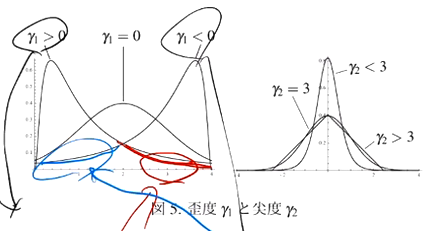
\includegraphics[width=14.0cm]{D_8/img_3.png}
    \end{center}
\end{figure}

%----------------------------------------------------------定義3.15
\noindent
\textbf{定義 3.15.} 標準化\\
$確率変数Xについて, E(X) = \mu, V(X) = \sigma^2 (\sigma > 0) とする. このとき, 変換$\\
\begin{align*}
    Z = \frac{X - \mu}{\sigma} \\
\end{align*}
$をXの \textbf{標準化(standardization)} とよぶ.$\\
%---------------以下補足
\begin{itembox}[l]{補足}
    \begin{align*}
         & E(X) = 0 \\
         & V(X) = 1 \\
    \end{align*}
\end{itembox}\\

%----------------------------------------------------------命題3.24
\noindent
\textbf{命題 3.24.} 標準化された確率変数の期待値, 分散\\
$標準化された, 確率変数Z の期待値 E(Z), 分散 V(Z) は以下で与えられる.$\\
\begin{align*}
    E(Z) = 0, \qquad V(Z) = 1 \\
\end{align*}
\begin{proof}
    \begin{align*}
        E(Z) & = E \left(\frac{X - \mu}{\sigma}\right) \\
             & = \frac{1}{\sigma}(E(X) - \mu) = 0      \\
    \end{align*}
    \begin{align*}
        V(Z) & = E \left(\left(\frac{X - \mu}{\sigma}\right)^2 \right) \\
             & = \frac{1}{\sigma^2}E((X - \mu)^2)                      \\
             & = \frac{\sigma^2}{\sigma^2} = 1                         \\
    \end{align*}
\end{proof}
$また, Zを変換した確率変数 X = \mu + \sigma Z の期待値 E(Z), 分散 V(Z) は以下で与えられる.$\\
\begin{align*}
    E(Z) = \mu, \qquad V(Z) = \sigma^2 \\
\end{align*}
\begin{proof}
    \begin{align*}
         & X = \mu + \sigma Z                                         \\
         & E(X) = \mu + \sigma E(Z) = \mu \qquad (\because E(Z) = 0)  \\
         & V(X) = \sigma^2 V(Z) = \sigma^2 \qquad (\because V(Z) = 1) \\
    \end{align*}
\end{proof}

\newpage
%----------------------------------------------------------定義3.16
\noindent
\textbf{定義 3.16.} スチューデント化\\
$確率変数Xについて, E(X) = \mu, V(X)=\sigma^2 (\sigma > 0) とする.このとき, 変換$\\
\begin{align*}
    T =\frac{X-\mu}{\sqrt{Y}} \\
\end{align*}
$をXの \textbf{スチューデント化(studentization)}とよぶ. ただし, Yは, Y \xrightarrow{P} \sigma^2 を満たす確率変数である.$\\

%----------------------------------------------------------定義3.17
\noindent
\textbf{定義 3.17.} \fbox{積率母関数}とキュムラント母関数\\
$確率変数Xについて, E(e^{tX}) < \infty が t の原点を含むある区間Iで成り立つとする.$
$この区間で定義されるtの関数$\\
\begin{align*}
    m_X(t) = E(e^{tX}) \qquad (t \in I) \\
\end{align*}
$をXの \textbf{積率母関数(moment \textcolor{red}{generating} function)}とよぶ.\; さらに,$\\
\begin{align*}
    \Psi_X(t) = log m_X(t) \qquad (t \in I) \\
\end{align*}
$を \textbf{キュムラント母関数(cumulant generating function)}とよぶ.$

%----------------------------------------------------------定理3.25
\noindent
\textbf{定理 3.25.} $確率変数Xについて, E(X^n) < \infty ならば, Xの積率母関数について以下が成り立つ. \; (使い方のみ)$\\
\begin{align*}
    \left. \frac{d^k}{dt^k}m_X(t) \right|_{t=0} = E(X^k) = \mu_k^{\prime} \qquad (k = 1,2, \dots n) \\
\end{align*}

%----------------------------------------------------------定理3.26
\noindent
\textbf{定理 3.26.} 積率母関数の一致性\\
$2つの確率変数 X_1, X_2に対して, 積率母関数m_{X_1}, m_{X_2} が存在すると仮定する.$
$このとき, 確率分布 P_{X_1}, P_{X_2} が一致するための必要十分条件は, 積率母関数m_{X_1}, m_{X_2} が一致することである.$\\
%---------------以下補足
\begin{itembox}[l]{補足}
    $P_{X_1} と P_{X_2} が一致 \leftrightarrow m_{X_1} と m_{X_1} が一致$\\
\end{itembox}\\

\newpage
%----------------------------------------------------------定理3.27
\noindent
\textbf{定理 3.27.} $確率変数Xについて, E(X^n) < \infty ならば, Xのキュムラント母関数に関して, 以下が成り立つ.$\\
\begin{align*}
    \left. \frac{d^k}{dt^k}\psi_X(t) \right|_{t=0} = \mathcal{K}_k \qquad (k = 1,2, \dots n) \\
\end{align*}

%----------------------------------------------------------命題3.28
\noindent
\textbf{命題 3.28.} 積率母関数, キュムラント母関数の線形変換\\
$a, b \in \mathbb{R} を定数とし, Y = aX+b とする. このとき, 確率変数X, Yの積率母関数, および, キュムラント母関数に関して, 以下が成り立つ.$\\
\begin{align*}
     & m_Y(t) =e^{bt}m_X(at)      \\
     & \psi_Y(t) =bt + \psi_X(at) \\
\end{align*}
\begin{proof}
    \begin{align*}
        m_Y(t) & = E(e^{ty})               \\
               & = E(e^{t(aX + b)})        \\
               & = E(e^{bt} \cdot e^{tax}) \\
               & = e^{bt} E(e^{tax})       \\
               & = e^{bt} m_X(at)          \\
    \end{align*}
\end{proof}

%----------------------------------------------------------命題3.29
\noindent
\textbf{命題 3.29.} 積率母関数とキュムラント母関数について, 以下の式が成り立つ.\\
\begin{align*}
     & \psi_X^{\prime}(0) = m_X^{\prime}(0) = E(X)                                     \\
     & \psi_X^{\prime \prime}(0) = m_X^{\prime \prime}(0) - (m_X^{\prime}(0))^2 = V(X) \\
\end{align*}
$ここでの, \prime および, \prime \prime はそれぞれ, 1階微分, 2階微分を表している.$\\

\newpage
%----------------------------------------------------------定理3.37
\noindent
\textbf{定理 3.37.} \textbf{マルコフの不等式(Markov's inequality)}\\
$h: \mathbb{R} \to \mathbb{R} を非負関数とする.\; 確率変数Xについて,E(h(X)) < \infty ならば, 任意の \epsilon > 0 に対して,$\\
\begin{align*}
    P(h(X) \geq \epsilon) \leq \frac{E(h(X))}{\epsilon} \\
\end{align*}
$が成り立つ.\; この不等式において, X を X - E(X) で置き換え, h(X) = x^2, \epsilon = a^2 とした$\\
\begin{align*}
    P(|X-E(X)| \geq a) \leq \frac{V(X)}{a^2} \\
\end{align*}
は\textbf{チェビシェフの不等式(Chebyshev's inequality)} とよばれる.\\
\begin{proof}
    \begin{align*}
        E(h(X)) = \int_{-\infty}^{\infty}h(x)f(x)dx & \geq \int_{h(x) \geq \epsilon}h(x)f_X(x)dx      \\
                                                    & \geq \int_{h(x) \geq \epsilon}\epsilon f_X(x)dx \\
                                                    & = \epsilon \int_{h(x) \geq \epsilon}f_X(x)dx    \\
                                                    & = \epsilon P(h(x) \geq \epsilon)                \\
    \end{align*}
\end{proof}

%----------------------------------------------------------定理3.38
\noindent
\textbf{定理 3.38.} \textbf{ジャンセンの不等式(Jensen's inequality)}\\
(凸関数と期待値の関係)\\
$g: \mathbb{R} \to \mathbb{R} を凸関数とする.\; 確率変数Xについて, E(X), E(g(X)) < \infty であれば,$\\
\begin{align*}
    g(E(X)) \leq E(g(X)) \\
\end{align*}
$が成り立つ.\; ここで, 区間Iで定義された実数関数gが凸関数であるとは, a,b \in I, t \in (0, 1)について,$\\
\begin{align*}
    g(ta + (1-t)b) \leq t(g(a)) + (1-t)g(b) \\
\end{align*}
が成り立つことである.\\

%----------------------------------------------------------定理3.39
\noindent
\textbf{定理 3.39.} \textbf{ヘルダーの不等式(holder's inequality)}\\
(コーシーシュワルツの一般形)\\
$確率変数X, Y について, E(|X|^p), E(|X|^q) < \infty であり, 1 < p < \infty, \frac{1}{p} + \frac{1}{q} = 1 であれば,$\\
\begin{align*}
    E(|XY|) \leq (E(|X|^p))^{1/p} (E(|Y|^q))^{1/q} \\
\end{align*}
$が成り立つ./; この不等式において, p = q = 2とした$\\
\begin{align*}
    \underline{(E(|XY|))^2 \leq E(X^2)E(Y^2)} \\
\end{align*}
$は, \textbf{コーシーシュワルツの不等式(Cauchy-Schwarz inequality)} とよばれる.$\\

%----------------------------------------------------------定理3.40
\noindent
\textbf{定理 3.40.} \textbf{ミンコフスキーの不等式(Minkowski's inequality)}\\
$確率変数X, Yについて, E(|X|^r), E(|Y|^r) < \infty であり, 1 \leq r < \infty であれば,$\\
\begin{align*}
    (E(|X + Y|^r))^{1/r} \leq (E(|X|^r))^{1/r} + (E(|Y|^r))^{1/r} \\
\end{align*}
が成り立つ.\\

%----------------------------------------------------------定理3.41
\noindent
\textbf{定理 3.41.} \textbf{リアプノフの不等式(Lyapunov's inequality)}\\
$確率変数Xについて, E(|X|^q) < \infty であり, 1 < p < q < \infty であれば,$\\
\begin{align*}
    (E(|X|^p))^{1/p} \leq (E(|X|^q))^{1/q} \\
\end{align*}
が成り立つ.\\
\end{document}
%本文ここまで=========================================================